%%%%%%%%%%%%%%%%%%%%%%%%%%%%%%%%%%%%%%%%%%%%%%%
%
% Template per Elaborato di Laurea
% DISI - Dipartimento di Ingegneria e Scienza dell’Informazione
%
% update 2015-09-10
%
% Per la generazione corretta del
% pdflatex nome_file.tex
% bibtex nome_file.aux
% pdflatex nome_file.tex
% pdflatex nome_file.tex
%
%%%%%%%%%%%%%%%%%%%%%%%%%%%%%%%%%%%%%%%%%%%%%%%

% formato FRONTE RETRO
\IfFileExists{./.draft}{
  \documentclass[epsfig,a4paper,11pt,titlepage,twoside,openany,draft]{book}
}{
  \documentclass[epsfig,a4paper,11pt,titlepage,twoside,openany]{book}
}

\usepackage{epsfig}
\usepackage{plain}
\usepackage{setspace}
\usepackage[paperheight=29.7cm,paperwidth=21cm,outer=1.5cm,inner=2.5cm,top=2cm,bottom=2cm]{geometry} % per definizione layout
\usepackage{titlesec} % per formato custom dei titoli dei capitoli
\usepackage[utf8x]{inputenc} % per Linux (richiede il pacchetto unicode);

\usepackage{acronym}
\usepackage{mdwlist}
\usepackage{easy-todo}
\usepackage{minted}
\usepackage{booktabs}
\usepackage{subcaption}

\usepackage{hyperref} % this should be the last imported

\acrodef{IPA}{International Publishers Association}
\acrodef{STM}{International Association of Scientific, Technical and Medical Publishers}
\acrodef{AAP}{Association of American Publishers}

\acrodef{MAG}{Microsoft Academic Graph}
\acrodef{pmf}{probability mass function}
\acrodef{cdf}{cumulative distribution function}
\acrodef{ccdf}{complementary cumulative distribution function}

\acrodef{SBN}{Standard Book Numbering}
\acrodef{ISO}{International Organization for Standardization}
\acrodef{DOI}{Document Object Identifier}
\acrodef{ISBN}{International Standard Book Number}
\acrodef{PMID}{PubMed Unique Identifier}

\acrodef{RDD}{Resilient Distributed Dataset}
\acrodef{CSV}{Comma-separated Values}

\singlespacing{}

\usepackage[english]{babel}

\begin{document}

  % nessuna numerazione
  \pagenumbering{gobble}
  % !TEX root = thesis.tex

\pagestyle{plain}

\thispagestyle{empty}

\begin{center}
  \begin{figure}[h!]
    \centerline{
\psfig{file=logo_unitn_black_center.eps,width=0.6\textwidth}}
  \end{figure}

  \vspace{2 cm}

  \LARGE{Department of Information Engineering and Computer Science\\}
  % \LARGE{Dipartimento di Ingegneria e Scienza dell’Informazione\\}

  \vspace{1 cm}
  \Large{Master Degree in Computer Science\\
    %Informatica
    %Ingegneria dell'Informazione e delle Comunicazioni
    %Ingegneria dell'Informazione e Organizzazione d'Impresa
    %Ingegneria Elettronica e delle Telecomunicazioni
  }

  \vspace{2 cm}
  \Large\textsc{Final Thesis\\}
  \vspace{1 cm}
  \Huge\textsc{An analysis of scholarly citations in Wikipedia\\}
  % \Large{\it{TODO: Sottotitolo (alcune volte lungo - opzionale)}}


  \vspace{2 cm}
  \begin{tabular*}{\textwidth}{ c @{\extracolsep{\fill}} c }
  \Large{Supervisor} & \Large{Graduand}\\
  \Large{Prof.\ Alberto Montresor}& \Large{Alessio Bogon}\\
  \end{tabular*}

  \vspace{2 cm}

  \Large{Academic year 2014/2015}

\end{center}


  \clearpage

%%%%%%%%%%%%%%%%%%%%%%%%%%%%%%%%%%%%%%%%%%%%%%%%%%%%%%%%%%%%%%%%%%%%%%%%%%
%%%%%%%%%%%%%%%%%%%%%%%%%%%%%%%%%%%%%%%%%%%%%%%%%%%%%%%%%%%%%%%%%%%%%%%%%%
%% Nota
%%%%%%%%%%%%%%%%%%%%%%%%%%%%%%%%%%%%%%%%%%%%%%%%%%%%%%%%%%%%%%%%%%%%%%%%%%
%% Sezione Ringraziamenti opzionale
%%%%%%%%%%%%%%%%%%%%%%%%%%%%%%%%%%%%%%%%%%%%%%%%%%%%%%%%%%%%%%%%%%%%%%%%%%
%%%%%%%%%%%%%%%%%%%%%%%%%%%%%%%%%%%%%%%%%%%%%%%%%%%%%%%%%%%%%%%%%%%%%%%%%%
  \thispagestyle{empty}

\begin{center}
  {\bf \Huge Ringraziamenti}
\end{center}

\vspace{4cm}


\emph{
  Thanks but no thanks.
}

  \clearpage
  \pagestyle{plain} % nessuna intestazione e pie pagina con numero al centro


  % inizio numerazione pagine in numeri arabi
  \mainmatter{}

%%%%%%%%%%%%%%%%%%%%%%%%%%%%%%%%%%%%%%%%%%%%%%%%%%%%%%%%%%%%%%%%%%%%%%%%%%
%%%%%%%%%%%%%%%%%%%%%%%%%%%%%%%%%%%%%%%%%%%%%%%%%%%%%%%%%%%%%%%%%%%%%%%%%%
%% Nota
%%%%%%%%%%%%%%%%%%%%%%%%%%%%%%%%%%%%%%%%%%%%%%%%%%%%%%%%%%%%%%%%%%%%%%%%%%
%% Si ricorda che il numero massimo di facciate e' 30.
%% Nel conteggio delle facciate sono incluse
%%   indice
%%   sommario
%%   capitoli
%% Dal conteggio delle facciate sono escluse
%%   frontespizio
%%   ringraziamenti
%%   allegati
%%%%%%%%%%%%%%%%%%%%%%%%%%%%%%%%%%%%%%%%%%%%%%%%%%%%%%%%%%%%%%%%%%%%%%%%%%
%%%%%%%%%%%%%%%%%%%%%%%%%%%%%%%%%%%%%%%%%%%%%%%%%%%%%%%%%%%%%%%%%%%%%%%%%%

    % indice
    \tableofcontents
    \clearpage



    % gruppo per definizone di successione capitoli senza interruzione di pagina
    \begingroup
      % nessuna interruzione di pagina tra capitoli
      % ridefinizione dei comandi di clear page
      %\renewcommand{\cleardoublepage}{}
      %\renewcommand{\clearpage}{}
      % redefinizione del formato del titolo del capitolo
      % da formato
      %   Capitolo X
      %   Titolo capitolo
      % a formato
      %   X   Titolo capitolo

      \titleformat{\chapter}
        {\normalfont\Huge\bfseries}{\thechapter}{1em}{}

      \titlespacing*{\chapter}{0pt}{0.59in}{0.02in}
      \titlespacing*{\section}{0pt}{0.20in}{0.02in}
      \titlespacing*{\subsection}{0pt}{0.10in}{0.02in}

      % sommario
      % !TEX root = thesis.tex

\chapter*{Introduction} % without page enumeration
\label{introduction}
\addcontentsline{toc}{chapter}{Introduction} % add me to the index anyway
Ever since Wikipedia was a few years old, there have been numerous academic studies about it.
Many of them analyze the production and reliability of the encyclopedia content, such as comparing the quality of articles to the Encyclopædia Britannica~\cite{Giles2005}.
Others have studied the social aspect, such as usage and administration.
For instance, Priedhorsky et al.~\cite{Priedhorsky2007} studied the population of Wikipedia contributors and the impact of false content in term of page visualizations.
Page visualizations plays an important role in recent studies:
for instance, McIver et al.~\cite{McIver2014} built a predictive model for the spread of influenza-like illness in the United States and Moat et al.~\cite{Moat2013} implemented a stock market moves strategy based on Wikipedia views.

It is very interesting to see that it is possible to predict behavior of many phenomena from the usage of Wikipedia.
Unfortunately, the page views dataset suffers from technical debt and it is not really suited for large-scale analysis.

We want to address this problem by providing a clean dataset which supports efficient analysis of page visualization.
The main difficulty for such task is given by the size of the dataset: its size is 4 728 GB for just the 2014, while the overall size up (from the 2008 to the 2015) is estimated to be 23 TB.
While the space requirements can be addressed, the computational power required is problematic.
Indeed we make use of the UniTN cluster infrastructure to split the work among multiple machines, exploiting the Apache Spark framework.

We also develop a framework to analyze Wikipedia dumps that can be used to extract arbitrary features, such as the publication identifiers for scholarly works appearing in articles.
With the extracted data, we analyze some of the patterns involving the behavior of such citations.

In particular, we analyze the quality of papers cited in the English Wikipedia in term of citations and we show how they tend to be more popular with respect to the ones released by journals like \emph{Science} or \emph{Nature}.
We also compare the most cited journals in Wikipedia with their ranking in the \ac{JCR}, showing that a correlation exists between the two.
Furthermore, we analyze how long it takes for the Wikipedia community to remove references that are not relevant for a certain article.
Indeed many of them are removed within one day after the insertion, possibly because of the effort made by contributors to maintain the quality of the articles.
An overview of the age of papers when they first appear shows that some authors look forward to insert their publication in Wikipedia articles as soon as they are released.


In Chapter~\ref{cha:background} we describe background concepts including publication identifiers, the Wikipedia structure and available resources, the Microsoft Academic Service that we exploit to understand links between academic papers and we briefly present the Apache Spark framework.
Chapter~\ref{cha:system_architecture} examines in detail the infrastructure used to recreate the page views dataset, the structure and problems of datasets and the implementation of the software developed.
In Chapter~\ref{cha:data_analysis} we present analyses regarding the behavior of scholarly citations in Wikipedia extracted using the developed software.
Chapter~\ref{cha:Contributions} shows the dataset and the programs developed and
in Chapter~\ref{cha:conclusion} we show what can be refined and we present some starting point for further research.

%%%%%%%%%%%%%%%%%%%%%%%%%%%%%%%%%%%%%%%%%%%%%%%%%%%%%%%%%%%%%%%%%%%%%%%%%%
%%%%%%%%%%%%%%%%%%%%%%%%%%%%%%%%%%%%%%%%%%%%%%%%%%%%%%%%%%%%%%%%%%%%%%%%%%
%% Nota
%%%%%%%%%%%%%%%%%%%%%%%%%%%%%%%%%%%%%%%%%%%%%%%%%%%%%%%%%%%%%%%%%%%%%%%%%%
%% Sommario e' un breve riassunto del lavoro svolto dove si descrive
%% l’obiettivo, l’oggetto della tesi, le metodologie e
%% le tecniche usate, i dati elaborati e la spiegazione delle conclusioni
%% alle quali siete arrivati.
%% Il sommario dell’elaborato consiste al massimo di 3 pagine e deve contenere le seguenti informazioni:
%%   contesto e motivazioni
%%   breve riassunto del problema affrontato
%%   tecniche utilizzate e/o sviluppate
%%   risultati raggiunti, sottolineando il contributo personale del laureando/a
%%%%%%%%%%%%%%%%%%%%%%%%%%%%%%%%%%%%%%%%%%%%%%%%%%%%%%%%%%%%%%%%%%%%%%%%%%
%%%%%%%%%%%%%%%%%%%%%%%%%%%%%%%%%%%%%%%%%%%%%%%%%%%%%%%%%%%%%%%%%%%%%%%%%%

      %%%%%%%%%%%%%%%%%%%%%%%%%%%%%%%%
      % lista dei capitoli
      %
      % \input oppure \include
      %
      \newpage
      % !TEX root = thesis.tex
\cleardoublepage{}
\chapter{Background}
\label{cha:background}

\section{Publication identifiers}
\label{sec:Publication identifiers}
In the scientific publishing environment that is increasingly moving online, identifiers of scholarly works plays a major role.
Indeed papers may be hosted in different places on the web and often there is more than one version available.
Identifiers are crucial to disambiguate articles that may share similar titles, or that  share the same set of authors because of homonymy.
There are many different types of identifier nowadays, some used more than others.
This research considers only four of them: \acs{DOI}, \acs{ISBN}, \emph{arXiv} and \acs{PMID}.
The choice is based on their popularity in Wikipedia and on technical reasons.

The \acf{DOI} system was created by the International DOI Foundation and was adopted as International Standard (ISO~26324) in 2012.
It originated in a joint initiative of three trade associations in the publishing industry: the \acf{IPA}, the \acf{STM} and the \acf{AAP}.
Millions of \ac{DOI} names have been assigned to date, through a growing federation of Registration Agencies worldwide.
For example, the Crossref application is used by more than 4\,800 publishers and societies to enable cross-citation of scholarly publications; the DataCite international federation of data centres uses the \ac{DOI} system; and the Entertainment Identifier Registry applies \ac{DOI} names to film and broadcast assets.

The \acf{ISBN} was developed by the \acf{ISO} and was published in 1970 as ISO 2108.
It originated from the \ac{SBN} code, a numeric commercial book identifier created by Gordon Foster, Emeritus Professor of Statistics at Trinity College, Dublin.
A unique \ac{ISBN} is assigned to every edition and variant of a book.

Wikipedia guidelines~\cite{wiki:doi_guideline} encourage the use of \acp{DOI} when available for journal sources, as well as the \ac{ISBN} references for book sources.

The \emph{arXiv} is a repository of electronic preprints of scientific papers in the fields of mathematics, physics, astronomy, computer science, quantitative biology, statistics, and quantitative finance, which can be accessed online.
In many fields of mathematics and physics, almost all scientific papers are self-archived on the arXiv.
At the time of writing, the archive counts more than one million articles.

Many references that appear in Wikipedia include the arXiv identifier, so it is included in our research.

Last but not least, the \acf{PMID} is a unique number assigned to each PubMed record.
PubMed is a free search engine accessing primarily the MEDLINE database of references and abstracts on life sciences and biomedical topics.
It provides quality control in scientific publishing. Only journals that meet PubMed's scientific standards are indexed.

In Wikipedia many journals citation in the medical field are inserted with the \ac{PMID} when available.



\section{Wikipedia}
\label{sec:wiki}
Wikipedia is a free-access, free-content Internet encyclopedia, supported and hosted by the non-profit Wikimedia Foundation.
Contributors can access the site and edit most of the articles.
Wikipedia is ranked among the ten most popular websites, and constitutes the Internet's largest and most popular general reference work~\cite{alexa}.
A peer review~\cite{Giles2005} of 42 science articles found in both Encyclopædia Britannica and Wikipedia was published in Nature in 2005, and found that Wikipedia's level of accuracy approached Encyclopædia Britannica's.
Although Wikipedia is arguably the most successful project of the Wikimedia Foundation, there are other projects under its umbrella.
Among them we can find: Wiktionary, a project to create a multilingual free content dictionary in every language; Wikibooks, which aims to build a collection of free e-book resources, including textbooks, language courses, manuals, and annotated public domain books; Wikiversity, a project dedicated to learning materials and learning communities, as well as research.

In this section we describe some of the entities that compose Wikipedia which are relevant to our analysis.

\paragraph{Pages}
The basic block of Wikipedia is the \emph{page}.
Pages are plain text document that can be customized using the wiki markup language, which is rendered when a user requests it.

A Wikipedia \emph{article} is a page that contains encyclopedic information.
A well-written encyclopedia article identifies a notable encyclopedic topic, summarizes that topic comprehensively, contains references to reliable sources and it links to other related topics.

\paragraph{Revisions}
Every time a \emph{contributor} edits a page, a new \emph{revision} is created.
It contains the text of the new version, as well as information about the contributor, the timestamp, the comment and others.

\paragraph{Namespaces}
Wikipedia pages are categorized under different \emph{namespaces}, according to their function.
To dictate the membership of a page, page titles are prefixed with the namespace followed by a colon.
For instance, the title of user pages is prefixed with the string \texttt{User:}.
The prefix is omitted for pages belonging to the main namespace, in which the encyclopedia articles appear.

At the time of writing, Wikipedia has 35 namespaces. The functional ones are 16 and they group pages that share the same purpose.
For instance, the ``Template'' contains templates devised to be included in articles and display information in an homogeneous way among articles.
Whenever a box is displayed inside an article, it has probably been generated by a template.
For every subject namespace (with the exception of ``Topic'') there is a corresponding ``Talk'' namespace.
In fact every page has a corresponding ``Talk'' page where users usually discuss about the content of the page and how to improve it.


Pages under the virtual namespaces ``Special'' and ``Media'' are not actually stored in the wikipedia database.
Special pages are created on demand by the MediaWiki software: for instance, \texttt{Special:Log} lists the log of all the activities on Wikipedia.
Files like images, videos and other assets live under the ``Media'' namespace.

\paragraph{Contributors}
Wikipedia \emph{contributors} can either be humans or bots.
Human contributors are usually referred with the name \emph{Wikipedians}.
Bots are usually employed to do repetitive and mundane tasks, such as correcting obvious typos, updating listified pages of categories or revert vandalisms.
At the time of writing the English Wikipedia has more than 27 millions users registered.
However, only a minority contributes regularly (0,4\% of users edited a page in the last month)~\cite{wiki:wikipedians}.

\paragraph{Redirects}
A \emph{redirect} is a page that has no content itself but sends the reader to another page, usually an article or a section of an article.
Redirects can be created for many reasons, among which:

\begin{itemize}
    \item Alternative names: an entity may be known as different names.
    For instance, the page \emph{Edison Arantes do Nascimento} is a redirect to \emph{Pelé}, which is the most appropriate article title according to Wikipedia rules.
    \item Abbreviations: some terms have an abbreviate form: for instance, \emph{US} is an abbreviation for \emph{United States}.
    According to Wikipedia guidelines, the title should be the the extended name, therefore a redirect from the abbreviation is created.
    \item Alternative spellings: there are names that refer to the same entity, for example \emph{Color} and \emph{Colour}.
    \item Likely misspellings: some names are commonly misspelled, and in order to not give an error page to the user, they redirects to the correctly spelled page.
    \item Technical reasons: some redirects are created because of technical issues.
    For example, there are redirects for pages with non-ASCII letters that have only ASCII letters in the title.
    Another reason is because of the software underneath Wikipedia.
    First versions of UseModWiki (the ancient engine used to power Wikipedia) needed pages to use the ``CamelCase'' convention for the name~\cite{wiki:camelcase}.
    This is not an issue anymore, but old page names are kept and they redirect to the non-camelcase name.
\end{itemize}

To mark a page as a redirect, it is necessary to include the string
\mintinline{text}{#redirect: [[Target]]} inside its source, where \emph{Target} is the page to which the reader will be redirected.

A recent study by Hill et al.~\cite{Hill2014} shows that redirect pages play an important role in Wikipedia, and must be taken into consideration when analyzing it.
They studied the work of Priedhorsky et al.~\cite{Priedhorsky2007}, where a surprisingly weak correlation between page edits and views have been found.
Hill et al.\ reproduced the analysis accounting for redirects and showed that the correlation is higher than the one discovered by the original authors.

The paper also discovered that 55\% of Wikipedia articles are redirects.
We have replicated their work using the latest data available and results are consistent with the original ones: at the time of writing, 59\% of Wikipedia articles are redirects (Table~\ref{tbl:redirects}).
This is particularly important in our analysis when we analyze how many users visited a page, because we must follow the redirects to get the correct count.

\begin{table}[t]
\centering
\begin{tabular}{@{}lrrr@{}}
\toprule
\multicolumn{1}{c}{\textbf{}} & \textbf{\# Redirects} & \textbf{\# Pages} & \textbf{Percentage of redirects} \\
\midrule
All namespaces    & 8350978                                & 37178009                               & 22,46\%             \\
Article namespace & 7075838                                & 11941857                               & 59,25\% \\
\bottomrule
\end{tabular}
\caption{Count of redirect pages in the English Wikipedia as of September 1st, 2015}
\label{tbl:redirects}
\end{table}

\paragraph{Vandalism}
Wikipedia articles can be edited by anyone --- there is no credential checking.
Changes are visible to everyone immediately, without any review cycle.
This comes at a cost: \emph{vandalism}.
Vandalism may come in different forms: pages may be subject to malevolent edits, deletions or moves.
Priedhorsky et al.~\cite{Priedhorsky2007} studied this phenomenon and recommended policies that may help to mitigate the problem.
The paper shows some blatant examples of vandalism: for example, Adam Curry allegedly altered pages about the history of podcasting in order to promote his role and diminish that of others, Jeffrey Seigenthaler's article stated falsely for months that he was involved in the John F. Kennedy assassination, and the comedian Stephen Colbert has even conducted humorous tutorials on how to vandalize Wikipedia.

Wikipedia currently uses various techniques to reduce its impact.
Pages that are considered ``at risk'' are protected in a way that only some users can edit the content.
Furthermore, administrators can prevent contributors from editing pages by banning them.
However, this can not solve the problem definitively because a contributor can change its IP address or create a new fake account.

%This is a serious problem for any analysis and requires some extra effort to reduce the impact it has in our results.

\section{Wikimedia page view statistics}
\label{sec:pagecounts}
Back in 2007, Domas Mituzas, a long-time volunteer database administrator for the Wikimedia Foundation, started generating statistics about the views of Wikimedia projects.
These statistics are now maintained by the Analytics Team\footnote{\url{https://www.mediawiki.org/wiki/Analytics}}.
The dataset contains the number of non-unique visitors for each page for all the Wikimedia projects, aggregated by hour.

A detailed explanation of the dataset is given in Section~\ref{sec:pagecounts}.
Unfortunately this dataset needs a lot of cleaning and, in order to be used effectively, needs to be reordered, as described in Section~\ref{sub:Sorting pagecounts}.

\section{Microsoft Academic Service}
\label{sec:mag}
Microsoft Academic Search is an experimental research service developed by Microsoft Research to explore how scholars, scientists, students, and practitioners find academic content, researchers, institutions, and activities.
The service indexed 83 million papers at the time of the writing of its technical report~\cite{Sinha2015} and, according to the authors, it achieved an above-95\% accuracy.
The service can also display the key relationships between and among subjects, content, and authors, highlighting the critical links that help define scientific research.

For these reasons, we use this service in our analysis.
The dataset is available under the name of \ac{MAG}\footnote{\url{http://research.microsoft.com/en-us/projects/mag/}}.
It contains 120\,887\,833 papers at the time of writing and some of them date back to 1800.
It also contains the references (in term of citations) between them, which is something of great value.

Unfortunately this source is not 100\% accurate, and in Section~\ref{sec:mag_dataset} are described some of its problems.


\section{Apache Spark}
The software developed in this work uses the Apache Spark framework to accelerate the computation of some datasets.
Apache Spark is an open source cluster computing framework originally developed in the AMPLab at University of California, Berkeley but was later donated to the Apache Software Foundation.
The basic building block of Spark is the \ac{RDD}, a logical collection of data partitioned across machines.
Spark includes various drivers to fetch data from different sources like databases (SQL and NO-SQL), HTTP, Amazon S3, HDFS, etc.
An \acs{RDD} can be created from various formats, such as \ac{CSV} files, or by applying transformation like \emph{map}, \emph{filter}, \emph{reduce} on other \acp{RDD}.

The value of Spark comes from the fact that transformations and other operations can be applied in parallel by multiple \emph{executors}.
An executor is a process spawned by a \emph{worker}, which is an instance of Spark running on a machine.
Furthermore, all the transformations are \emph{lazy} in that they do not compute the result right away.
Instead, they are computed only when needed: this design enables Spark to run more efficiently.
For example, it can realize that a dataset created through a \emph{map} will be used in a \emph{reduce} and return only the result of the reduce to the driver (i.e.\ the process running the application), rather than the larger mapped dataset.

One can run a Spark program on a single machine exploiting the available cores, but the real power of Spark comes when a cluster is available.
It is sufficient to start the cluster manager on the \emph{master} host and the worker on the \emph{slaves} to exploit the processing power of the whole cluster.
In the end, however, some tuning of the application is needed to make the most out of the available resources.

      \newpage
      % !TEX root = thesis.tex

\chapter{System architecture}
\label{cha:system_architecture}

\section{Datasets}
\label{sec:datasets}

\subsection{Wikimedia dumps}
The Wikimedia foundation creates a dump of the publicly available data of Wikipedia and all WMF projects on a regular basis.
English Wikipedia is dumped once a month, while smaller projects are often dumped twice a month.
The Wikimedia datasets used for our research are the one released the 1st of September 2015\footnote{\url{https://dumps.wikimedia.org/enwiki/20150901/}}.

\begin{table}[]
\centering
\caption{Size of wikipedia dump files.}
\label{tbl:wikidumps_size}
\begin{tabular}{@{}lrrr@{}}
\multicolumn{1}{c}{\textbf{}} & \textbf{Compressed size} & \textbf{Uncompressed size} & \textbf{Compression ratio} \\ \midrule
Pages dump              &     105.9 GB &   13\,387.9 GB &  0.79 \% \\
Category links table    &       1.7 GB &        12.1 GB & 13.77 \% \\
Page table              &       1.3 GB &         4.2 GB & 30.84 \% \\
Redirect table          &      96.9 MB &       364.3 MB & 26.60 \%
\end{tabular}
\end{table}

\paragraph{Pages XML dump}
The most important dataset for our purposes is the dump of all the pages, which include every revision created so far.
As you can see in Table~\ref{tbl:wikidumps_size}, this dataset is the most large: its uncompressed size is 13\,387.9 GB\@.
It is divided in 187 XML files compressed with 7zip, each of them containing several pages.
An extract of a dump is shown in Listing~\ref{lst:page_xml_extract}.
Every file contains a ``preamble'' with various metadata.
We can find the XML Schema location, the name of the project inside the \mintinline{xml}{<siteinfo>} tag, the list of namespaces up-to-date.
This is followed by a sequence of \mintinline{xml}{<page>} elements, each of them describing a Wikimedia page: its title, the namespace and the id.
Notice that if the title contains a space, it is not replaced by an underscore.
After that there is sequence of \mintinline{xml}{<revision>} tags.
A revision is identified by an identifier, and usually have also reference (parent id) to the previous reference.
\todo{show that page revision graph is cyclic}
If this is the first revision of a page, this field will be left empty.
There are some other metadata fields, like the timestamp, the contributor and the comment.
Finally, we can find the actual source of the page in plain text format.

Thanks to the structure of the file, it is easy to analyze the file iterating over the XML elements without loading it entirely in memory.

\begin{listing}[]
    \inputminted[breaklines=true]{xml}{assets/page_xml_extract.xml}
    \caption{Extract of a dump XML document.}
    \label{lst:page_xml_extract}
\end{listing}

\paragraph{Database dumps}
There are other datasets from Wikipedia that come in form of SQL dump files generated from the MySQL database powering Wikipedia.
There is a minor discrepancy between the convention used the XML dumps and these SQL dumps regarding the title of a page.
While in the former it is not normalized in any way, in the latter spaces are replaced with underscores.
It is important to keep it in mind when analyzing these datasets.

The tables used in this project are three: redirects, pages and category links.
The \emph{redirect} dump has all the information needed for the redirect mechanism offered by the MediaWiki software.
It contains all the information about page redirects, in particular the id of the page from which the redirect starts, the title of the target page and its namespace.
It also contains other information, but they are not worth of description for our purposes.

The \emph{page} table contains up-to-date information about all the pages.
The relevant features the page id, the namespace and the page title.
There are other columns that are used by the MediaWiki software, such as the restrictions or the timestamp of the last edit, but they are not relevant for our analysis.

The \emph{categorylinks} dump contain the membership of pages to categories.
Every row represent a link between a page and a category.
Indeed we can find the id of the page, the name of the category and the type of link (for example, the link ``page'' denotes that a page belongs to a category, while ``subcat'' is used for categories belonging to other categories).
Other fields denotes the timestamp of the link creation and indexing metadata.

\section{Wikimedia pagecounts}
The Wikimedia page view statistics dataset, aka \emph{pagecounts-raw}, can be downloaded directly from the Wikimedia downloads directory\footnote{\url{https://dumps.wikimedia.org/other/pagecounts-raw/}}.
It is a fairly huge source of data: the dataset compressed size referring to the 2014 is 866 GB distributed in 8756 files.
It is generated by the Wikimedia Squid caching servers: every time a reader request a page a log entry is created and the page is served.
Notice that the cache server does not know if the requested page is an article, a special page, a redirect or even if it exists.
Furthermore, if a page request contain spaces, these are replaced with underscores, because the MediaWiki software uses this convention.

It consists of many files, each of them containing the aggregated page view for a specific hour.
Files use a CSV dialect with \emph{spaces} as separators and they are compressed using the gzip format.
The encoding of this file is not documented.
Many of them seem to use UTF-8, while others ISO-8859-2. % chktex 8
We use the first decoder for all the files, and whenever a Unicode endpoint cannot be found, we replace it with the official \textbf{U+FFFD REPLACEMENT CHARACTER}.

Every file is named according the following format:
\begin{verbatim}
    pagecounts-{year}{month}{day}-{hour}{minute}{second}.gz
\end{verbatim}
The content consists of four columns: the Wikimedia project, the requested page, the number of requests for that page in the last hour, and the size of the response.
The Wikimedia project name has of two parts.
The first is the abbreviation of the language of the project (e.g. \textbf{en} for English Wikimedia projects, \textbf{it} for Italian, etc.) and the second is the abbreviation of the name of the project prefixed by a dot (e.g. \textbf{.b} for wikibooks, \textbf{.d} for wiktionary, etc.).
In case of Wikipedia projects, the second part is omitted, and only the language abbreviation is kept.
Notice that this field is not always in lowercase: this is caused by clients that request url with mixed case letters.
A normalization is therefore required.

The second column, the requested page, is usually escaped by client browser replacing special bytes with an \textbf{\%xx} string, where \textbf{xx} is the hex representation, as per RFC 1808~\cite{rfc1808}.
It is necessary to decode this representation, since different client software can decide to encode or not certain characters.
For instances, client can decide to encode the page named \textbf{New\_Year's\_Day} as \textbf{New\_Year's\_Day} of \textbf{New\_Year\%27s\_Eve}.
This must be taken in consideration, since they refer to the same entity.

The third and the fourth column contains respectively the number of times the page has been served in the hour, and the size of bytes transferred to the clients.
This last field is not relevant for our purposes, but it will be kept because it may be useful for some other research.

In Listing~\ref{lst:pagecounts_extract} is shown an sample from the dump of the first hour of 2014.
The first line is straight forward: the page \textbf{Chomsky} has been seen once, and the size of the response was 98\,938 bytes.
The second line exhibit an example of encoding: the actual name of the page was \textbf{Chomsky–Schützenberger\_theorem} and all the non-ascii character plus the dash have been replaced with their hexadecimal representation.

\begin{listing}[]
    \inputminted[breaklines=true]{xml}{assets/pagecounts_extract_first_hour.txt}
    \caption{Extract from the first hour of the 2014 pagecounts-raw dataset (\textbf{pagecounts-20140101-000000.gz})}
    \label{lst:pagecounts_extract}
\end{listing}

\section{Microsoft academic graph}
\label{sec:mag_dataset}
Microsoft release a dump of the dataset powering Microsoft Academic Search in form of CSV files, compressed with zip.
A brief overview of the size of the dataset is shown in Table~\ref{tbl:mag_size}.

\begin{table}[]
\centering
\caption{Size of Microsoft academic graph dataset files.}
\label{tbl:mag_size}
\begin{tabular}{@{}lrrr@{}}
\multicolumn{1}{c}{\textbf{}} & \textbf{Compressed size} & \textbf{Uncompressed size} & \textbf{Compression ratio} \\ \midrule
Papers table                &      9.0 GB &    27.4 GB & 32.71 \% \\
Paper references table      &      7.4 GB &    18.1 GB & 41.02 \% \\
Paper keywords table        &      1.8 GB &     5.3 GB & 34.51 \%
\end{tabular}
\end{table}

There are many entities in this dataset, and in our analysis we make use of most of them.

The \emph{Papers} listing contains information like the name of the paper, the publication date, its \ac{DOI} (if available), the journal or the conference where it appeared on.
There is a total of 120\,887\,833 papers, but only 35\,039\,319 of them contains a \ac{DOI} record (28.99\%) and, most important, only 33\,345\,644 of them have exactly one \ac{DOI} (27.58\%).
The fact that two papers share the same \ac{DOI} should be sought in the method used by Microsoft to index them.
It is important that a good percentage of papers have this identifier because our analysis relies on the fact that we can match publications that appear in Wikipedia, and this is done by matching the \ac{DOI} of a paper.

There is another important listing in this dataset, the \emph{PaperReferences} dump.
This table contains just two columns: the referring and the referred paper ids.

Finally, there are other files that contains information about the \emph{Journals}, \emph{Conferences}, \emph{Authors}, \emph{Keywords}, etc.


\todo{Explain that the ``conferences'' dataset is extremely biased: it seems that there are only compsci conferences}


\section{Software}
\label{sec:software}
\subsection{Sorting pagecounts}
\label{sub:Sorting pagecounts}
A great amount of time has been spent on the pagecounts dataset.
Currently it is partitioned by the timestamp of each hour.
This representation is useful if you need to get the views for a certain hour, but as soon as you want to get the views for an article in the 2014 it is simply not feasible.
Indeed, you would need to sequentially scan all the 8756 files, decompressing them on the fly.
Also, you could not perform any search optimization based on bisection, since the content inside the files is not ordered and because the content is not normalized.
Therefore we decided to reorganize this dataset, normalizing the content and sorting it by project, page and timestamp, without losing information.

The program written for this purposes is a Spark job, using the Python programming language.
Apache Spark is an open source cluster computing framework originally developed in the AMPLab at University of California, Berkeley but was later donated to the Apache Software Foundation.
The basic building block of Spark is the \ac{RDD}, a logical collection of data partitioned across machines.
\ac{RDD} can be created from existing data sources, such as \ac{CSV} files, or by applying transformation like \emph{map}, \emph{filter}, \emph{reduce} on other \acp{RDD}.
Their peculiarity is that transformations can be applied in parallel by multiple \emph{workers}.

The idea is to normalize the content of the input files, then repartition the entities (i.e.\ the tuples containing the statistics for a given page in a project in a specific hour) using the ordering key.
Finally, every output partition is re-ordered locally and the result is saved into a different CSV file.

Our program will indeed create an \ac{RDD} for every input file.
This is implicitly decompressed upon read operations.
Each line of the file is normalized: the project field is converted to lowercase and the page title is decoded according to RFC 1308~\cite{rfc1808}.
This transformation may cause multiple lines that refer to the same entity.
\todo{explain why}
Therefore it is necessary to merge these lines into one, summing the count of the views and the bytes transferred.
A \emph{key function} is also defined: it takes a tuple of the form \mintinline{python}{(timestamp, project, page, counts, bytes)} and returns the \mintinline{python}{(project, page)} key.

To repartition the entities, we need to fix the number of output partition.
This value fixed to the number of input files, let's say $N$.

Now we want to create a \emph{range partitioner}, a function that takes a tuple and returns the index of the new partition it belongs to.
Notice that Python implicitly defines an ordering between tuples by comparing their fields one at a time.
To create this function, we take an ordered sample of the keys of the first \ac{RDD} and enumerate it.
This enumeration is in fact a mapping between a key (project, page) and a partition index.
When looking for the partition for a new tuple $t$, it is sufficient to return the index corresponding to the last key which is less or equal to $t$.
Since the enumeration is ordered, the search can be optimized using the bisect algorithm.

At this point the \emph{union} of the input \acp{RDD} is repartitioned using this function, resulting in a coarse-sorted dataset.
The last operation needed is to sort tuples of each partition locally.
Values of these partition (i.e.\ tuples containing the timestamp, count and bytes) are also sorted by timestamp.
This results in a new \ac{RDD} normalized and sorted by \mintinline{python}{(page, project, timestamp)}.
The last step is to save the result in a CSV file.
The dataset is actually split in multiple gzipped CSV files because we want to avoid to merge partitions.

Since this job is highly parallelizable, we exploit the UniTN Cisca cluster described \todo{describe it}.
Spark includes a cluster management which makes this operation more or less painless.
It is sufficient to start the Spark executable on the workstations and wait for them to connect to the master server.
Once they are ready, it is sufficient to launch the job on the master, and it automatically splits the tasks between the workers.


\todo{Spark, python libs, sqlite}


\section{Infrastructure}
\label{sec:infrastructure}
\todo{My pc, ``adige'', unitn cluster}

      \newpage
      % !TEX root = thesis.tex

\chapter{Data analysis}
\label{cha:data_analysis}
The datasets created allow to perform some measurement regarding the use of scholarly works in the English Wikipedia.
\todo{TODO\@: other statistics? Maybe some that use the pagecounts?}

\section{Wikipedia articles}
\subsection{Where do identifiers appear in a Wikipedia article?}

\subsection{How many sections Wikipedia articles have?}

\subsection{Which are the most common sections in Wikipedia articles?}

\section{Papers in Wikipedia}
This section analyzes the use of papers in wikipedia.

\subsection{Incoming citations distribution}
The distribution of scholarly citations has been studied many times by the scientific community.
The problem is to understand the law that describes the \emph{distribution of citations} of papers, namely the distribution of the number of papers $N(x)$ that have been cited $x$ times.
Redner~\cite{Redner1998} suggested that this distribution has a large-$x$ power law decay $N(x) \sim x^{-\alpha}$ \todo{explain some more of that article}.

Fig.~\ref{fig:incoming_citations_loglog} compares the distribution of citations of all the papers known to the MAG (circa 120 millions) and the ones whose \ac{DOI} appears in Wikipedia (circa 389 thousands).
The number of incoming citation for a paper is determined using the \ac{MAG} dataset.
Notice that the only identifier available in the \ac{MAG} is the \ac{DOI}, hence only the papers found in Wikipedia which have a \ac{DOI} are considered.
This accounts for the 28\% of the identifiers found.
Furthermore, from this set of papers we removed the ones that appears to be ``non-valid'' in the \ac{MAG} dataset, namely the ones that have more than one \ac{DOI}.
The amount of papers considered at the end is the 17\% of the identifiers found in Wikipedia.

From the graph we can only see that both the distribution follow some kind of power law.
It is more interesting to analyze the \ac{CCDF} of the two series.
In our case, the \ac{CCDF}, or \emph{tail distribution}, expresses the percentage of papers $\bar{F}(x)$ that have more than $x$ citations.

From Fig.~\ref{fig:incoming_citations_ccdf_1000}~and~\ref{fig:incoming_citations_ccdf_100} we can see that papers appearing in Wikipedia tend to have many more incoming citations with respect to a random paper taken from all the available ones.
For instance, the 74\% of papers in Wikipedia have at least 10 incoming citations, while only the 13\% of papers have at least 10 incoming citations.
A plausible explanation is that users tend to insert papers with a higher rank in term of incoming citations, rather than ones with less impact on the scientific community.
\todo{Regarding the ``All papers'' serie, should we limit only papers having DOIs?}
% see https://en.wikipedia.org/wiki/User:ProteinBoxBot.


\begin{figure}[h]
\centering
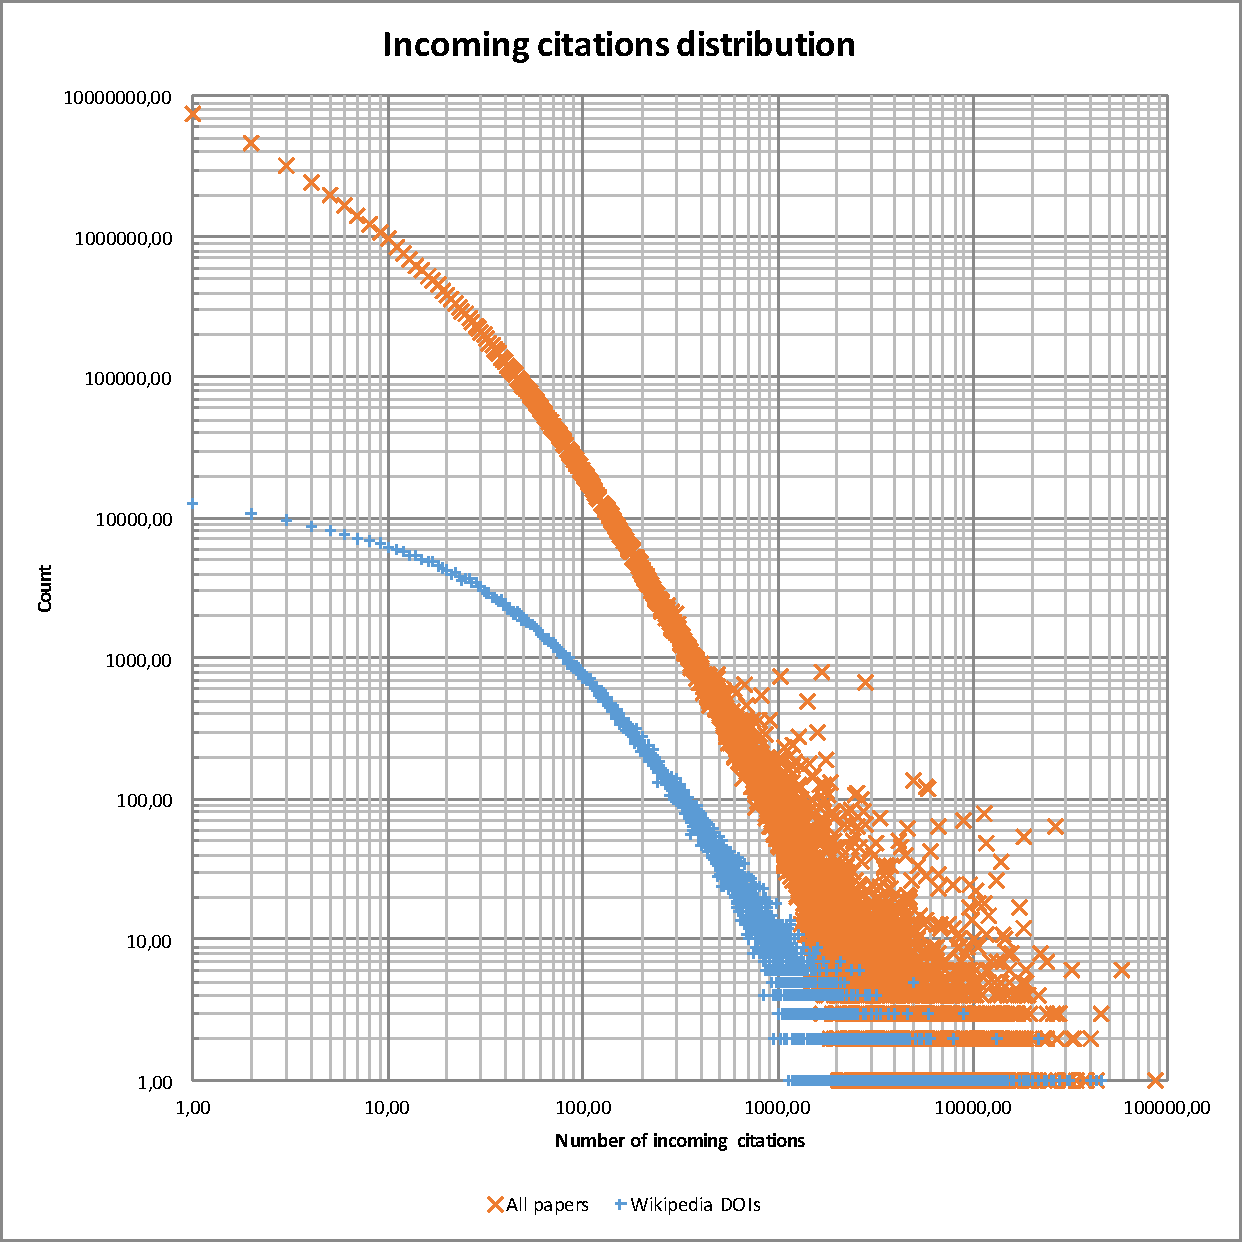
\includegraphics[keepaspectratio=true, width=\textwidth]{assets/incoming_cits_loglog}
\caption{Incoming citations distribution of papers appearing in the \emph{mag} datasets and the ones appearing only in English Wikipedia, on a log-log scale.}
\label{fig:incoming_citations_loglog}
\end{figure}

\begin{figure}[h]
\centering
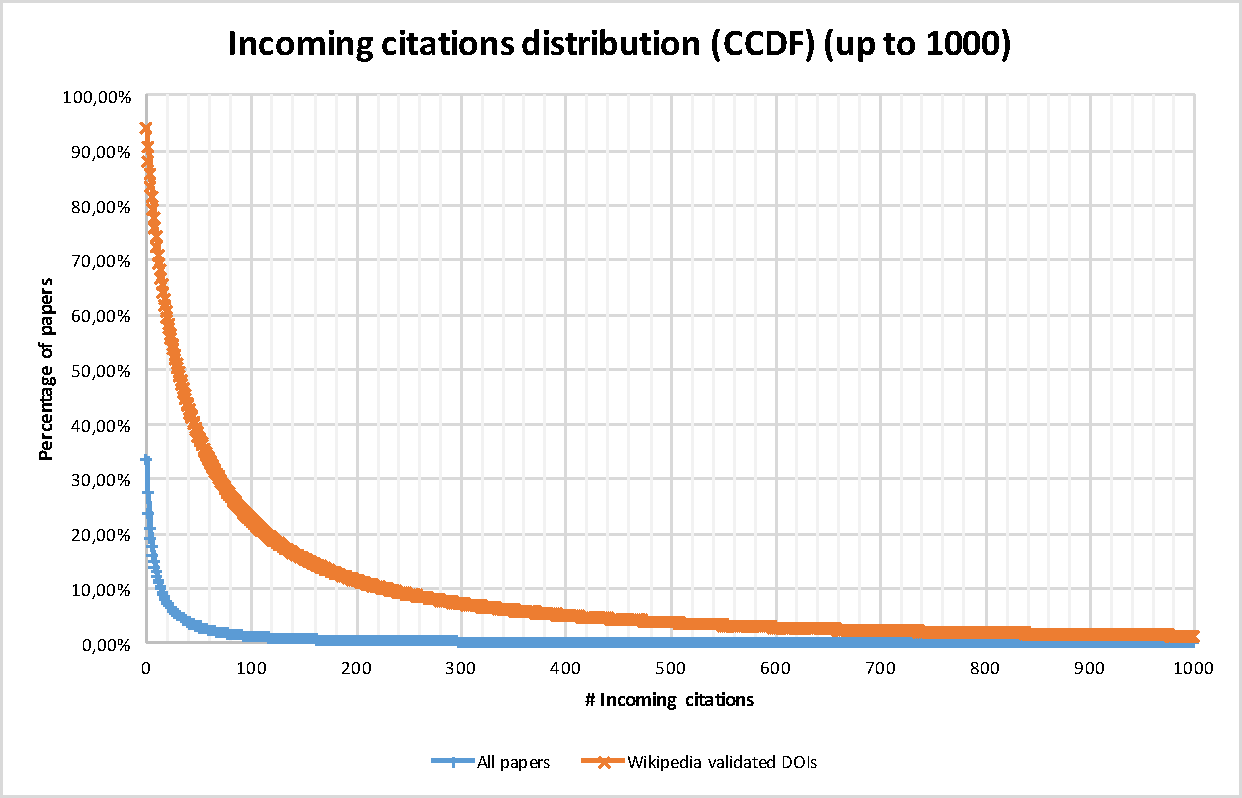
\includegraphics[keepaspectratio=true, width=\textwidth]{assets/incoming_cits_ccdf_1000}
\caption{Complementary cumulative distribution function of the first 100 incoming citations of papers appearing in the \emph{mag} datasets and the ones appearing only in English Wikipedia.}
\label{fig:incoming_citations_ccdf_1000}
\end{figure}

\begin{figure}[h]
\centering
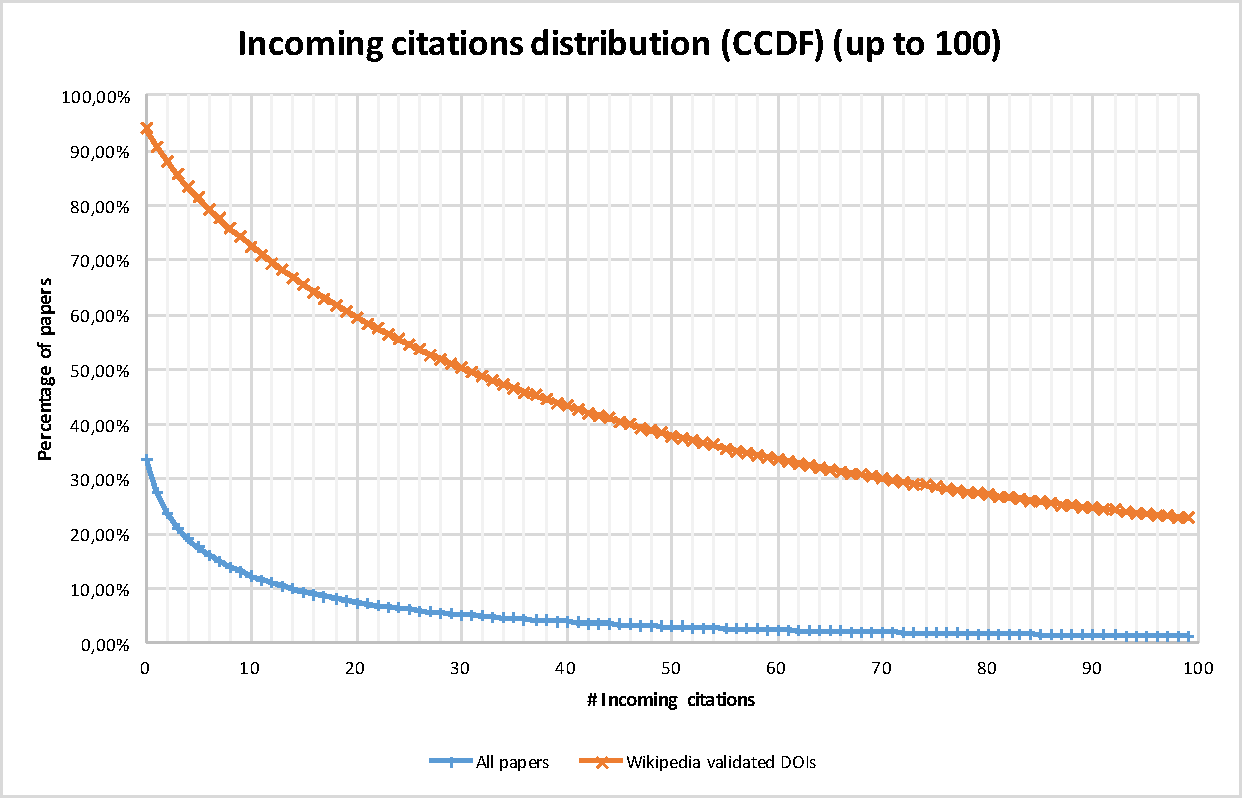
\includegraphics[keepaspectratio=true, width=\textwidth]{assets/incoming_cits_ccdf_100}
\caption{Complementary cumulative distribution function of the first 100 incoming citations of papers appearing in the \emph{mag} datasets and the ones appearing only in English Wikipedia.}
\label{fig:incoming_citations_ccdf_100}
\end{figure}

\subsection{Age of identifiers at first appearance}
Another interesting information to analyze is the age of the papers when they first appear in Wikipedia.
Fig.~\ref{fig:age_of_papers_at_first_appearance} shows the distribution of the age of papers when they are inserted on Wikipedia for the first time.
In theory there should not be negative values, because this would mean that an identifier appears in Wikipedia before the paper is published.
In practice this happens because the \ac{MAG} dataset is not 100\% accurate, and some publication dates may contain errors.
We have investigated this problem, and it seems to be caused by how Microsoft extracts the publication date of a paper.
It appears that if a paper is published online on a certain date, and it is also released after in a journal, Microsoft consider the date of the journal the publication date.
However, only the 3,12\% of the \acp{DOI} extracted have a negative age, so the effect of the error is arguably quite marginal.

It is interesting to see that many \acp{DOI} are inserted in Wikipedia few days after their publication (Fig.~\ref{fig:age_of_papers_at_first_appearance_zoom}).
We have analyzed some of these cases, and it appears that that some authors insert the identifier of their paper as soon as it has been published.

Finally, to give a scale to this numbers, Fig.~\ref{fig:age_of_papers_at_first_appearance_cdf} measure is the \ac{CDF} of the serie, namely what is the percentage $F(x)$ of paper identifiers inserted in Wikipedia at most $x$ days after their publication.
\todo{conclude, somehow}

% Notes:
% Kamil Crater (doi 10.1126/science.1190990) has been added by the author as soon as possible. \url{https://en.wikipedia.org/w/index.php?title=Kamil_Crater&diff=next&oldid=375884625}

\begin{figure}[h]
\centering
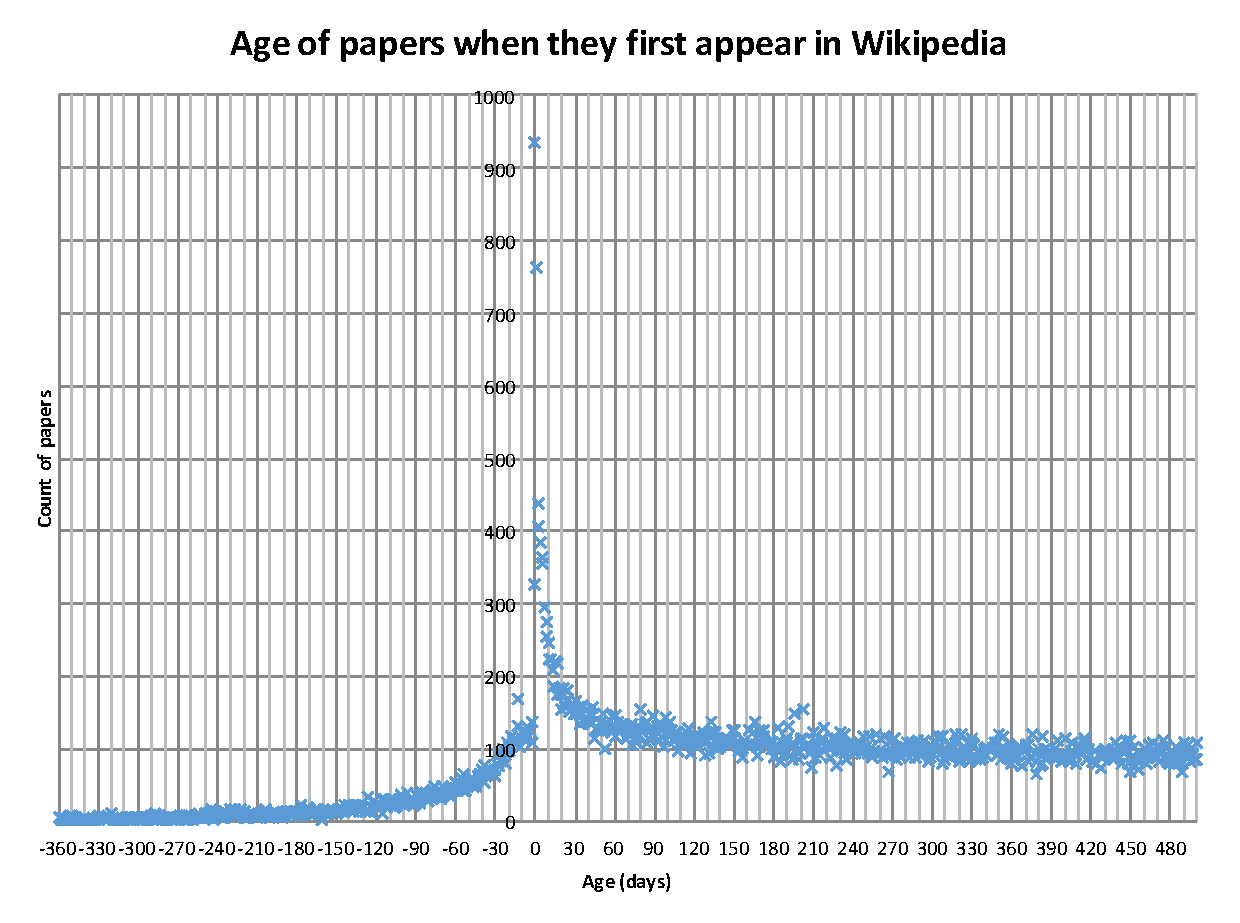
\includegraphics[keepaspectratio=true, width=\textwidth]{assets/age_of_papers_at_first_appearance}
\caption{Distribution of the age of papers when their DOI appear for the first time on Wikipedia.}
\label{fig:age_of_papers_at_first_appearance}
\end{figure}

\begin{figure}[h]
\centering
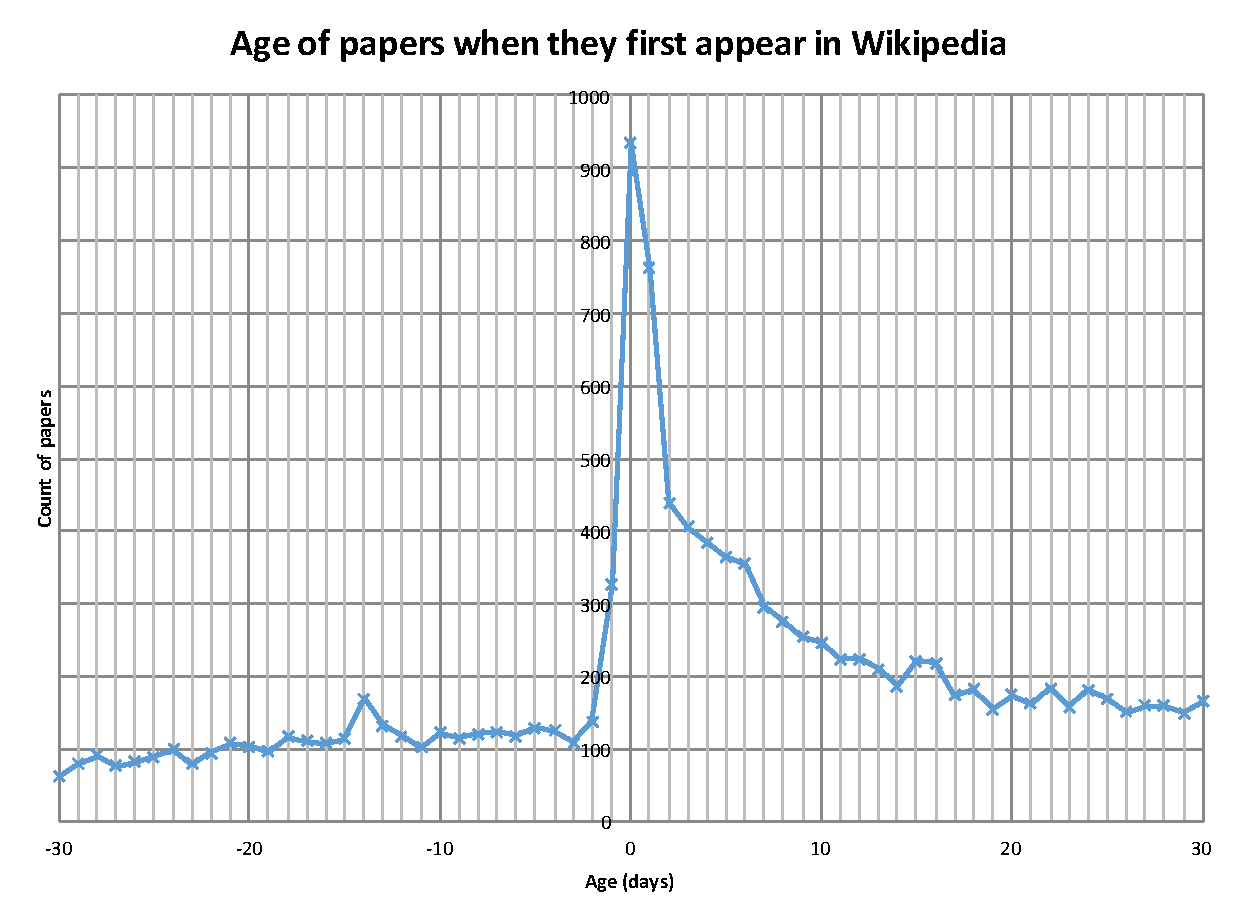
\includegraphics[keepaspectratio=true, width=\textwidth]{assets/age_of_papers_at_first_appearance_-30+30}
\caption{Distribution of the age of papers when their DOI appear for the first time on Wikipedia, showing only ages between $[-30, 30]$ days.}
\label{fig:age_of_papers_at_first_appearance_zoom}
\end{figure}

\begin{figure}[h]
\centering
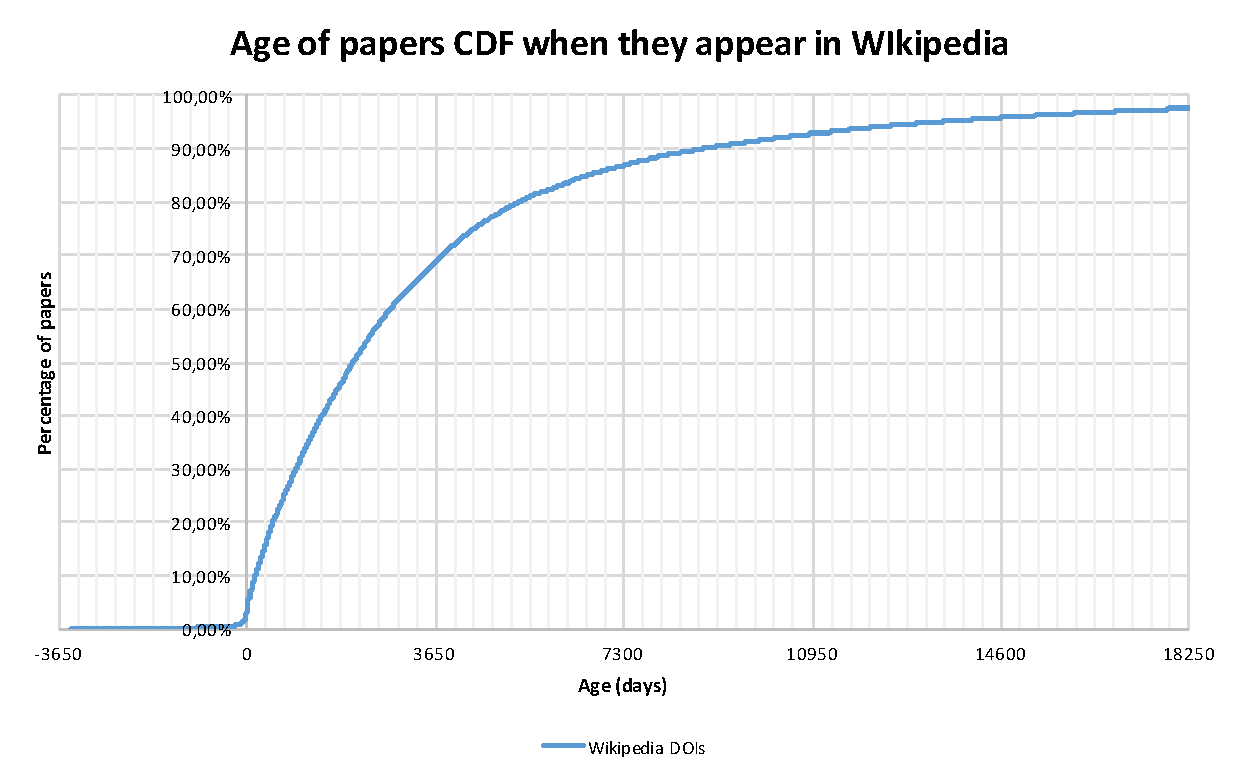
\includegraphics[keepaspectratio=true, width=\textwidth]{assets/age_of_papers_at_first_appearance_cdf}
\caption{todo}
\label{fig:age_of_papers_at_first_appearance_cdf}
\end{figure}

\subsection{Identifiers lifetime}
todo: show graph of identifier insertions in time
analizza la persistenza degli identifier inseriti e rimossi

fare la average della persistenza degli identifier escludendo la coda
\subsection{Publication date distribution}
\subsection{Top cited journals by views}

      \newpage
      % !TEX root = thesis.tex
\cleardoublepage{}
\chapter{Contributions}
\label{cha:Contributions}
In this chapter we describe the dataset generated and the software developed which are made available for further works.

\section{Page views ordered by project, article}
\label{sec:contrib_datasets_pagecounts}
This dataset~\cite{Bogon2016} has been generated starting from the Wikimedia's pagecounts-raw dataset using the program described in Section~\ref{sub:Sorting pagecounts}.
It contains the page view statistics for all the Wikimedia projects in the year 2014, ordered by $(project, page, timestamp)$.
We plan to generate this collection also for the remaining years.
The size is 4\,728 GB (428 GB compressed) split across 67056 files.

The content of the dataset is formatted in CSV, where each row describes the number of requests for a page of in a specific hour.
The fields are the following:
\begin{itemize}
    \item project: the name of the Wikimedia project, lowercase
    \item page: the name of the page, URL-escaped
    \item timestamp: the timestamp of the hour, (format \mintinline{text}{%Y%m%d-%H%M%S})
    \item count: the number of times the page has been requested
    \item bytes: the number of bytes transferred
\end{itemize}

We also released a Python library, \emph{pagecounts-search}\footnote{\url{https://github.com/youtux/pagecounts-search}}, to search through this source of information.
It can be used either as a library inside another project or directly as a command line tool.

This dataset has been created because we found that the original page views dataset is not well suited for most of the purposes.
Indeed some of the cited works use dodge the problem by restricting the number of pages to be analyzed or by using alternative sources.

\section{Wikipedia extraction framework}
\label{sub:contrib_programs_framework}
The \emph{wikidump}\footnote{\url{https://github.com/youtux/wikidump}} framework started as a project to extract some features from the Wikipedia dumps described in Section~\ref{sec:Wikipedia dumps}.
It uses libraries developed by Aaron Halfaker to analyze the XML structure and to extract identifiers from the text using regular expressions and parsers.
We have modified the identifiers extraction module to improve its performance, and it is currently waiting to be merged in the \emph{python-mwrefs}\footnote{\url{https://github.com/mediawiki-utilities/python-mwrefs}} library.

The framework allows the extraction of features such as the history of publication identifiers (\ac{ISBN}, \ac{DOI}, \ac{PMID}, \emph{arXiv}), statistics about the pages' sections, interlinks between pages, etc.

It analyzes the dumps by iterating over the elements of the XML file, without keeping them in memory in order to avoid exhaustion.
It also automatically decompresses the input file if needed and the user can choose to enable the compression of the output file.
Because of the nature of the dataset, the program can be used to analyze more files in parallel.

      \newpage
      % !TEX root = thesis.tex

\chapter{Conclusion and further work}
\label{cha:conclusion}
TODO

      \nocite{*}

    \endgroup


    % bibliografia in formato bibtex
    %
    % aggiunta del capitolo nell'indice
    \addcontentsline{toc}{chapter}{Bibliography}
    % stile con ordinamento alfabetico in funzione degli autori
    \bibliographystyle{plain}
    \bibliography{biblio}
%%%%%%%%%%%%%%%%%%%%%%%%%%%%%%%%%%%%%%%%%%%%%%%%%%%%%%%%%%%%%%%%%%%%%%%%%%
%%%%%%%%%%%%%%%%%%%%%%%%%%%%%%%%%%%%%%%%%%%%%%%%%%%%%%%%%%%%%%%%%%%%%%%%%%
%% Nota
%%%%%%%%%%%%%%%%%%%%%%%%%%%%%%%%%%%%%%%%%%%%%%%%%%%%%%%%%%%%%%%%%%%%%%%%%%
%% Nella bibliografia devono essere riportati tutte le fonti consultate
%% per lo svolgimento della tesi. La bibliografia deve essere redatta
%% in ordine alfabetico sul cognome del primo autore.
%%
%% La forma della citazione bibliografica va inserita secondo la fonte utilizzata:
%%
%% LIBRI
%% Cognome e iniziale del nome autore/autori, la data di edizione, titolo, casa editrice, eventuale numero dell’edizione.
%%
%% ARTICOLI DI RIVISTA
%% Cognome e iniziale del nome autore/autori, titolo articolo, titolo rivista, volume, numero, numero di pagine.
%%
%% ARTICOLI DI CONFERENZA
%% Cognome e iniziale del nome autore/autori (anno), titolo articolo, titolo conferenza, luogo della conferenza (città e paese), date della conferenza, numero di pagine.
%%
%% SITOGRAFIA
%% La sitografia contiene un elenco di indirizzi Web consultati e disposti in ordine alfabetico.
%% E’ necessario:
%%   Copiare la URL (l’indirizzo web) specifica della pagina consultata
%%   Se disponibile, indicare il cognome e nome dell’autore, il titolo ed eventuale sottotitolo del testo
%%   Se disponibile, inserire la data di ultima consultazione della risorsa (gg/mm/aaaa).
%%%%%%%%%%%%%%%%%%%%%%%%%%%%%%%%%%%%%%%%%%%%%%%%%%%%%%%%%%%%%%%%%%%%%%%%%%
%%%%%%%%%%%%%%%%%%%%%%%%%%%%%%%%%%%%%%%%%%%%%%%%%%%%%%%%%%%%%%%%%%%%%%%%%%


    \titleformat{\chapter}
        {\normalfont\Huge\bfseries}{Appendix \thechapter}{1em}{}
    % sezione Allegati - opzionale
    \appendix
    % \chapter{Titolo primo allegato}
%
% Lorem ipsum dolor sit amet, consectetur adipiscing elit. Donec sed nunc orci. Aliquam nec nisl vitae sapien pulvinar dictum quis non urna. Suspendisse at dui a erat aliquam vestibulum. Quisque ultrices pellentesque pellentesque. Pellentesque egestas quam sed blandit tempus. Sed congue nec risus posuere euismod. Maecenas ut lacus id mauris sagittis egestas a eu dui. Class aptent taciti sociosqu ad litora torquent per conubia nostra, per inceptos himenaeos. Pellentesque at ultrices tellus. Ut eu purus eget sem iaculis ultricies sed non lorem. Curabitur gravida dui eget ex vestibulum venenatis. Phasellus gravida tellus velit, non eleifend justo lobortis eget.
%
% \section{Titolo}
% Lorem ipsum dolor sit amet, consectetur adipiscing elit. Donec sed nunc orci. Aliquam nec nisl vitae sapien pulvinar dictum quis non urna. Suspendisse at dui a erat aliquam vestibulum. Quisque ultrices pellentesque pellentesque. Pellentesque egestas quam sed blandit tempus. Sed congue nec risus posuere euismod. Maecenas ut lacus id mauris sagittis egestas a eu dui. Class aptent taciti sociosqu ad litora torquent per conubia nostra, per inceptos himenaeos. Pellentesque at ultrices tellus. Ut eu purus eget sem iaculis ultricies sed non lorem. Curabitur gravida dui eget ex vestibulum venenatis. Phasellus gravida tellus velit, non eleifend justo lobortis eget.
%
% \subsection{Sottotitolo}
% Lorem ipsum dolor sit amet, consectetur adipiscing elit. Donec sed nunc orci. Aliquam nec nisl vitae sapien pulvinar dictum quis non urna. Suspendisse at dui a erat aliquam vestibulum. Quisque ultrices pellentesque pellentesque. Pellentesque egestas quam sed blandit tempus. Sed congue nec risus posuere euismod. Maecenas ut lacus id mauris sagittis egestas a eu dui. Class aptent taciti sociosqu ad litora torquent per conubia nostra, per inceptos himenaeos. Pellentesque at ultrices tellus. Ut eu purus eget sem iaculis ultricies sed non lorem. Curabitur gravida dui eget ex vestibulum venenatis. Phasellus gravida tellus velit, non eleifend justo lobortis eget.
%
%
% \chapter{Titolo secondo allegato}
%
% Lorem ipsum dolor sit amet, consectetur adipiscing elit. Donec sed nunc orci. Aliquam nec nisl vitae sapien pulvinar dictum quis non urna. Suspendisse at dui a erat aliquam vestibulum. Quisque ultrices pellentesque pellentesque. Pellentesque egestas quam sed blandit tempus. Sed congue nec risus posuere euismod. Maecenas ut lacus id mauris sagittis egestas a eu dui. Class aptent taciti sociosqu ad litora torquent per conubia nostra, per inceptos himenaeos. Pellentesque at ultrices tellus. Ut eu purus eget sem iaculis ultricies sed non lorem. Curabitur gravida dui eget ex vestibulum venenatis. Phasellus gravida tellus velit, non eleifend justo lobortis eget.
%
% \section{Titolo}
% Lorem ipsum dolor sit amet, consectetur adipiscing elit. Donec sed nunc orci. Aliquam nec nisl vitae sapien pulvinar dictum quis non urna. Suspendisse at dui a erat aliquam vestibulum. Quisque ultrices pellentesque pellentesque. Pellentesque egestas quam sed blandit tempus. Sed congue nec risus posuere euismod. Maecenas ut lacus id mauris sagittis egestas a eu dui. Class aptent taciti sociosqu ad litora torquent per conubia nostra, per inceptos himenaeos. Pellentesque at ultrices tellus. Ut eu purus eget sem iaculis ultricies sed non lorem. Curabitur gravida dui eget ex vestibulum venenatis. Phasellus gravida tellus velit, non eleifend justo lobortis eget.
%
% \subsection{Sottotitolo}
% Lorem ipsum dolor sit amet, consectetur adipiscing elit. Donec sed nunc orci. Aliquam nec nisl vitae sapien pulvinar dictum quis non urna. Suspendisse at dui a erat aliquam vestibulum. Quisque ultrices pellentesque pellentesque. Pellentesque egestas quam sed blandit tempus. Sed congue nec risus posuere euismod. Maecenas ut lacus id mauris sagittis egestas a eu dui. Class aptent taciti sociosqu ad litora torquent per conubia nostra, per inceptos himenaeos. Pellentesque at ultrices tellus. Ut eu purus eget sem iaculis ultricies sed non lorem. Curabitur gravida dui eget ex vestibulum venenatis. Phasellus gravida tellus velit, non eleifend justo lobortis eget.
%
%


\end{document}
